\DocumentMetadata{
  pdfversion=2.0,
  lang=es-MX,
  pdfstandard=ua-2
}

\documentclass{sener2025}

\addbibresource{referencias.bib}

% --- Metadatos PDF/UA (Accesibilidad Universal) ---
\hypersetup{
  pdftitle={Documento de Prueba SENER},
  pdfauthor={Dirección General de Planeación Energética},
  pdfsubject={Prueba de funcionalidades del template},
  pdfkeywords={prueba; template; LaTeX; SENER},
  pdfcreationdate={D:20251212120000},
  pdfversion={1}
}

% --- Metadatos del Documento ---
\title{Documento de Prueba SENER}
\subtitle{Verificación de funcionalidades del template}
\author{Dirección General de Planeación Energética}
\date{12 de diciembre de 2025}
\institucion{Secretaría de Energía (SENER)}
\unidad{Unidad de Planeación y Transición Energética}
\setDocumentoCorto{PruebaSENER}
\palabrasclave{prueba; template; LaTeX; SENER}
\version{1.0}

\begin{document}

\portadafondo

\tableofcontents
\newpage

\listafiguras
\newpage

\listatablas
\newpage

\begin{resumenejecutivo}
Este documento de prueba verifica que todas las funcionalidades del template SENER funcionen correctamente, incluyendo fuentes, enlaces, tablas, figuras y elementos especiales.
\end{resumenejecutivo}

\begin{datosclave}
  \begin{itemize}
    \item Template funcional al 100\%
    \item Fuentes Noto Sans y Patria cargadas
    \item Enlaces clicables en índices
    \item Tablas con formato institucional
  \end{itemize}
\end{datosclave}

\section{Prueba de Fuentes y Formato}

Este texto usa la fuente principal Noto Sans. \textbf{Este texto está en negritas.} \textit{Este texto está en cursivas.}

{\patriafont Este texto usa la fuente Patria para títulos.}

\subsection{Prueba de Enlaces}

Los enlaces en el índice de contenidos, figuras y tablas deben ser clicables y dirigir a la sección correspondiente.

\subsubsection{Prueba de Listas}

Lista con viñetas:
\begin{itemize}
  \item Primer elemento
  \item Segundo elemento con \textbf{texto en negritas}
  \item Tercer elemento con \textit{texto en cursivas}
\end{itemize}

\section{Prueba de Tablas}

\begin{tabladorado}
  \caption{Tabla de prueba con formato institucional}
  \label{tab:prueba_formato}
  \begin{tabular}{p{4cm}p{3cm}p{3cm}p{3cm}}
    \toprule
    \rowcolor{gobmxDorado} \encabezadodorado{\textbf{Concepto}} & \encabezadodorado{\textbf{2023}} & \encabezadodorado{\textbf{2024}} & \encabezadodorado{\textbf{2025}} \\
    \midrule
    \textbf{Capacidad Total} & 85,000 & 87,500 & 90,000 \\
    \textbf{Renovables} & 25,000 & 30,000 & 35,000 \\
    \textbf{Convencionales} & 60,000 & 57,500 & 55,000 \\
    \bottomrule
  \end{tabular}
\end{tabladorado}
\fuente{Elaboración propia para pruebas del template}

\section{Prueba de Figuras}

\begin{figure}[H]
  \centering
  \pdftooltip{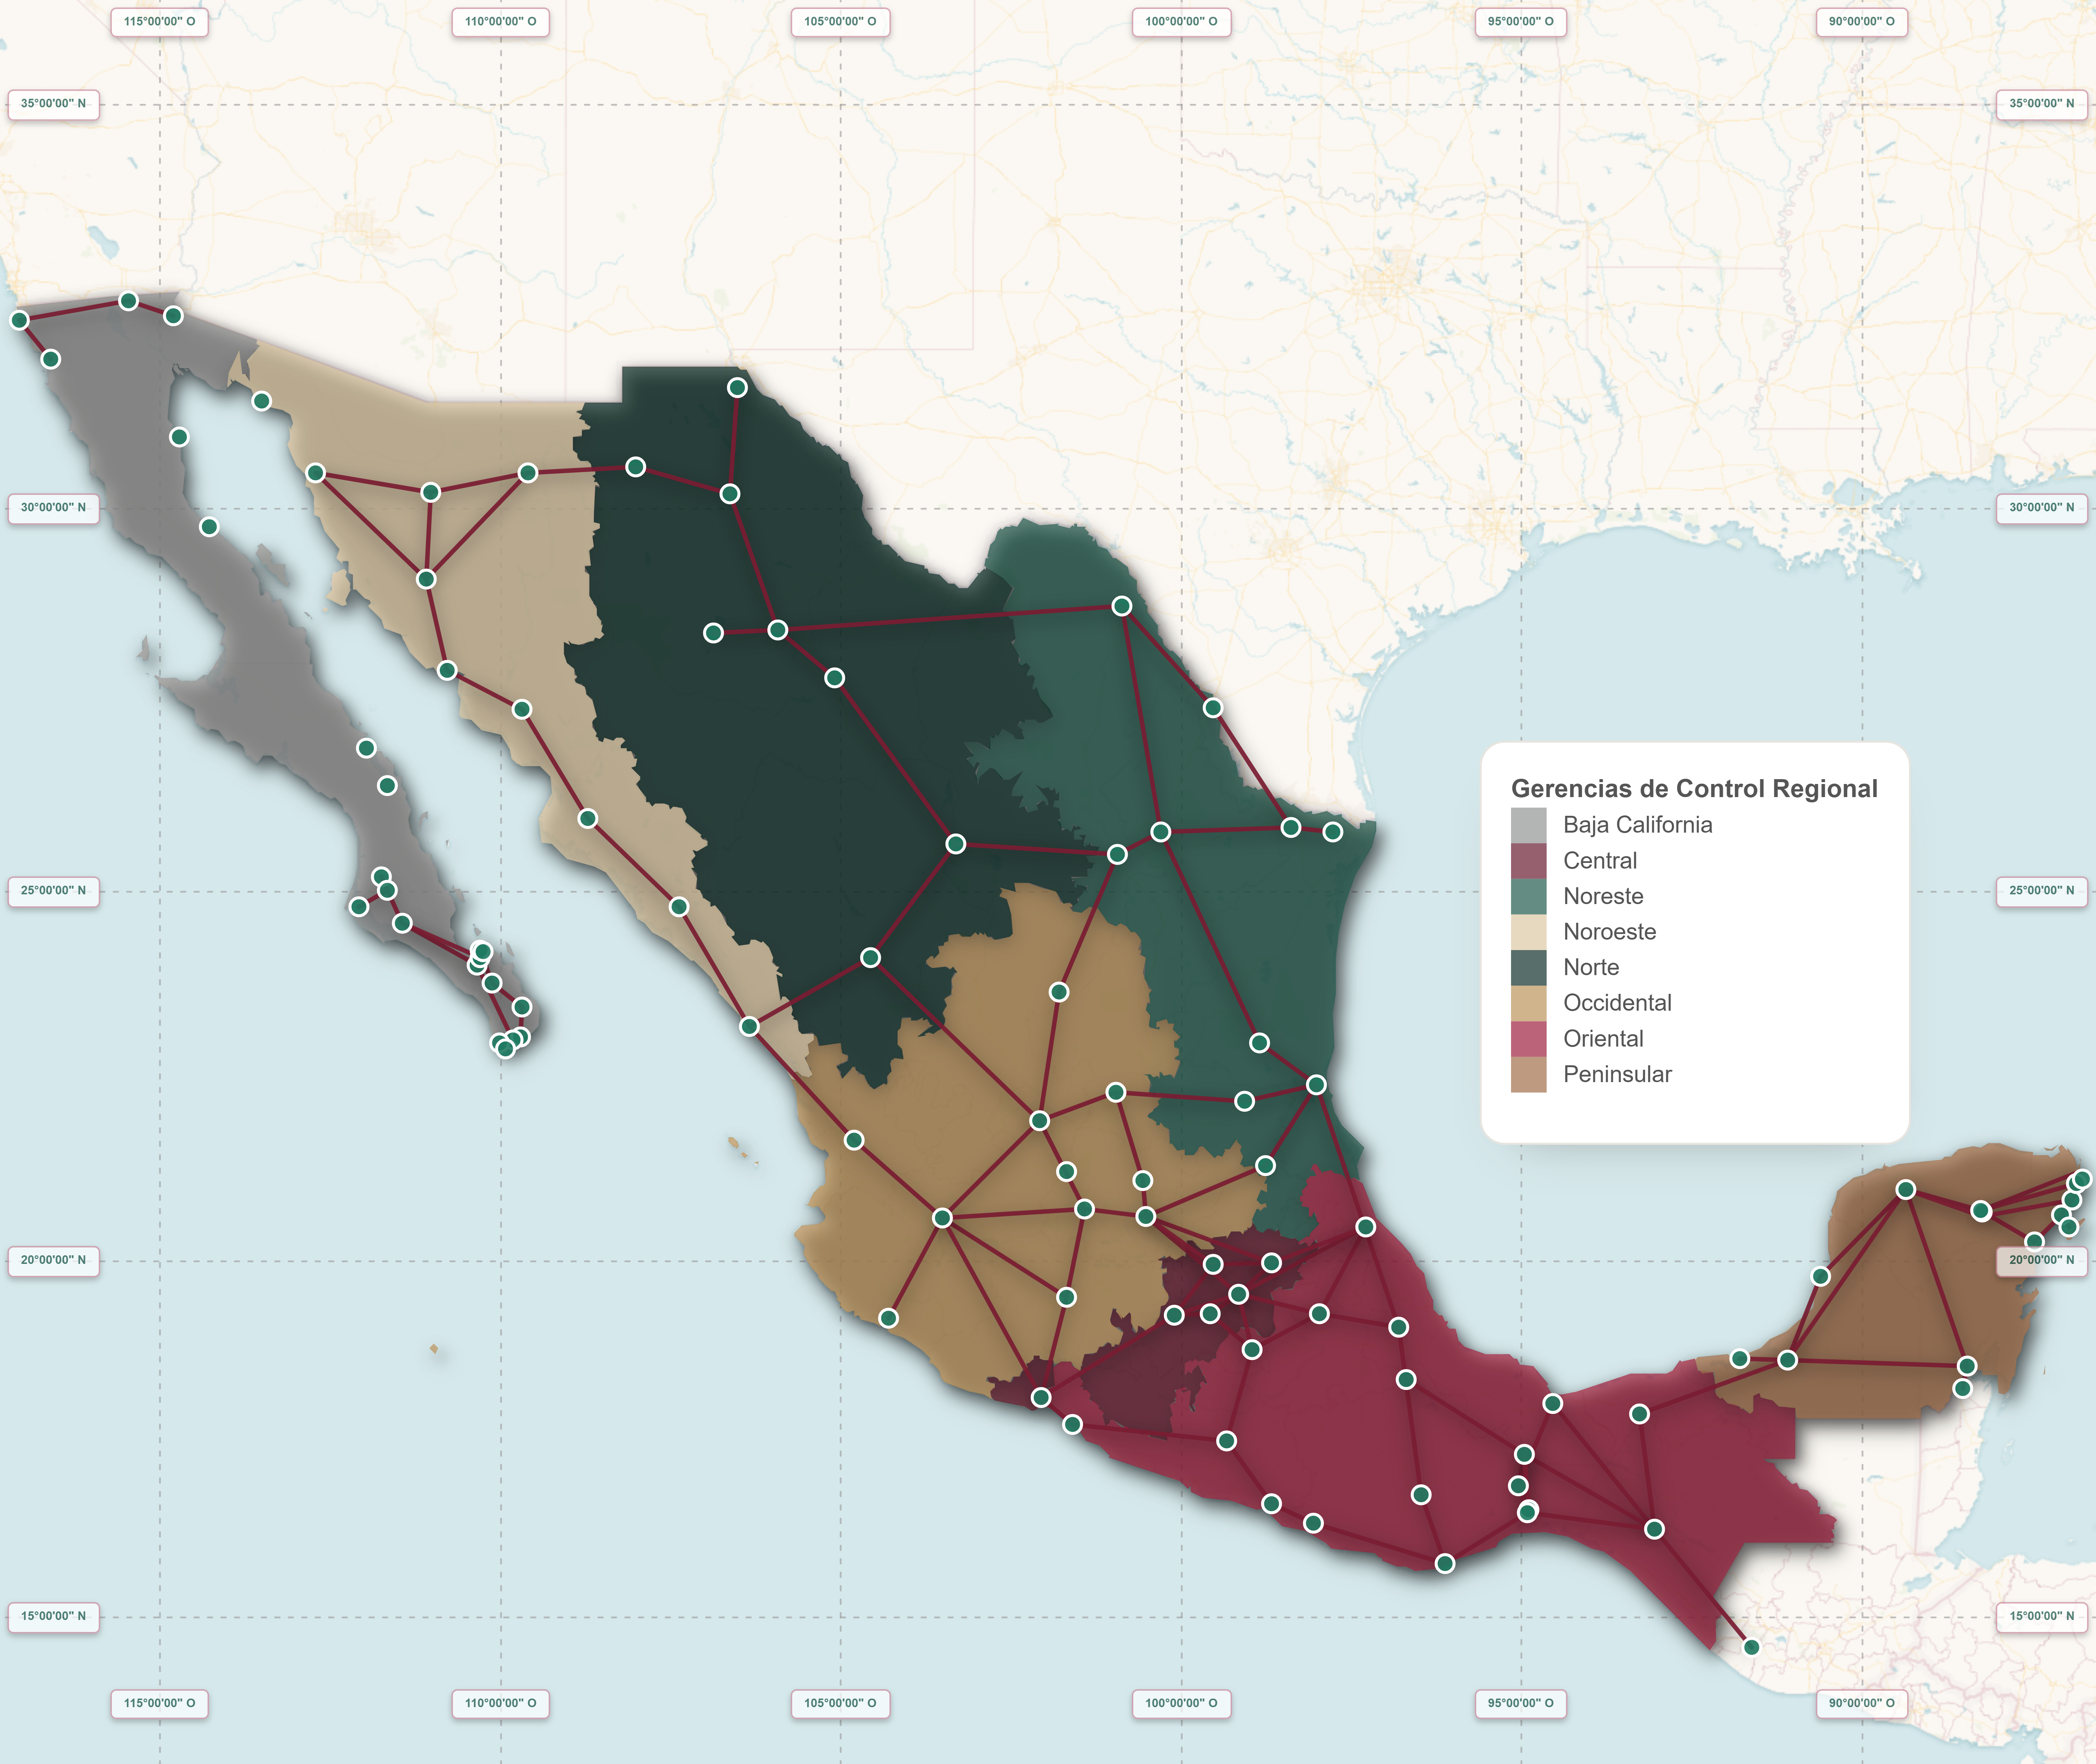
\includegraphics[width=0.6\textwidth]{img/graficos/figura_2_1.png}}{Gráfica de prueba que muestra datos de ejemplo para verificar el funcionamiento del template}
  \caption{Figura de prueba del template SENER}
  \label{fig:prueba_template}
\end{figure}
\fuente{Imagen de prueba del template}

\section{Prueba de Elementos Especiales}

\begin{destacado}
Este es un texto destacado que debe aparecer con formato especial.
\end{destacado}

\begin{ejemplo}[title={Ejemplo de Uso}]
Este es un ejemplo de cómo usar los elementos especiales del template:
\begin{itemize}
  \item Usar \texttt{tabladorado} para tablas institucionales
  \item Usar \texttt{destacado} para texto importante
  \item Usar \texttt{ejemplo} para casos de uso
\end{itemize}
\end{ejemplo}

\begin{calloutTip}[Consejo]
Los enlaces en los índices deben funcionar correctamente. Si no funcionan, verificar la configuración de hyperref.
\end{calloutTip}

\begin{calloutWarning}[Advertencia]
Las fuentes personalizadas requieren XeLaTeX para funcionar correctamente.
\end{calloutWarning}

\section{Verificación de Enlaces}

Esta sección verifica que los enlaces funcionen:
\begin{itemize}
  \item Referencia a tabla: Ver Tabla~\ref{tab:prueba_formato}
  \item Referencia a figura: Ver Figura~\ref{fig:prueba_template}
  \item Los enlaces en el índice deben ser clicables
\end{itemize}

\section*{Glosario}
\addcontentsline{toc}{section}{Glosario}

\entradaGlosario{Template}{Plantilla prediseñada para documentos LaTeX}
\entradaGlosario{XeLaTeX}{Motor de compilación LaTeX que soporta fuentes modernas}

\section*{Siglas y Acrónimos}
\addcontentsline{toc}{section}{Siglas y Acrónimos}

\entradaSigla{SENER}{Secretaría de Energía}
\entradaSigla{PDF}{Portable Document Format}

\contraportada{
\textbf{\textcolor{gobmxDorado}{Elaboración:}}\\
Equipo de Desarrollo de Templates\\
Dirección de Sistemas\\[0.5cm]

\textbf{\textcolor{gobmxDorado}{Contacto:}}\\
Secretaría de Energía\\
Jalapa 20, Col. Roma Norte\\
Ciudad de México, C.P. 06700\\
Tel: (55) 5000-6000\\
\textbf{\textcolor{gobmxGuinda}{www.gob.mx/sener}}
}

\end{document}